\documentclass[12pt]{article}
\usepackage[margin=1.0in]{geometry}
\usepackage[utf8]{inputenc}
\usepackage[T1]{fontenc}
\usepackage{lmodern}
\usepackage[spanish]{babel}
\usepackage{amsmath}
\usepackage{graphicx}

\title{Response to the referee}

\begin{document}

\date{}
\maketitle

\section{Global Comments}

\subsection{Variation with the viewing angle}

The problematic of anisotropy is only studied from Sect3.4, the former sections consider global quantities (spectral shapes, escape fractions, etc...). This is ok only if there is NO anisotropy induced by rotation, which is not obvious, a priori. You should make it clear from the beginning, telling that you will investigate anisotropy at the end of the paper only, because you checked that lya properties are isotropic, at least in the range of parameters that you investigated so far.\\


\textbf{ We have decide to study in this paper the case in which there is No anisotropy. The part concerning the off-center emission is going to be presented in a later study\\}

As explained in sect 3.4, rotation kills the spherical symmetry of your problem, and the rotation axis defines a preferential direction. We could expect some variation of the emerging flux, the lyman-alpha escape fraction, and the spectral shape, with viewing angle. From Fig8, it seems that the flux is the same in all directions for spherical distributions of sources. This important result is not enough emphasized.\\

\textbf{We do not find the flux variation with the viewing angle and now as highlighted in the new text we emphasize more this new result, also we made a new plot Figure 5 in the paper, showing this results for both distributions (homogeneous/central) and for optical depth $\tau_{H}=10^{5}$ we choose these models because this are the ones 
that are more sensitive to rotation.\\}

Do you see any difference in the spectral shape with viewing angle ? To illustrate this point, it would be interesting to build a 2D plot as you did on Fig 5, but replace Nb scat in ordinates by the viewing angle μ. We could immediatly see if there is an evolution of the shape with viewing angle or not. If you find NO evolution of the Lya shape with viewing angle, I think that it is an interesting counter-intuitive result, that you should advertise more.\\

\textbf{Thanks very much for this recommendation we made this new plot and we do find variations in the morphology of the line due to variations in the viewing angle. We have restructure the paper this new plots now correspond to figure 2 & 3 in the paper.  Also we emphasize this results in the results, discussion and conclusion sections.\\}

What about the variation of lya escape fraction with viewing angle ? I propose that in the beginning of Sect.3 Results, you first emphasize that, maybe counter-intuitively, you did not find any variation of the Lya properties with viewing angle, so you will present first angle average lya properties, and you will come back to the anisotropy problematic only at the end on the paper.\\

\textbf{As escape fraction depends on the number of scatterings and this is invariant for different viewing angles the escape fraction does not change with the viewing angle. (MAKE A PLOT AND EXPLAIN THIS BETTER)
}


\section*{Outflow + Rotation}

We want to study the pure effect of rotation on the spectra, off course it would
be interesting to study the effect of rotation on systems with outflows, this paper
is under preparation by M.C Remolina-Gutierrez et al.  

\section*{Details}

\subsection*{Introduction}

With Orsi et al 2012, please cite also Garel et al 2012. With Zheng&Wallace 2013, please cite also Behrens et al 2014.\\

\textit{This changes were performed.}
\subsection*{Fig.1}

I guess that the spectra presented in Fig1 are integrated over all directions, right ? You should describe explicitly how you build them. You could skip the x notation in absciss, as it is not used in the discussion, whereas the velocity is used to compare to FWHM, on Fig2.\\

\textbf{Now this figure is the Fig.4 in the paper. what we did was to fix a viewing angle in this case $\theta= \pi/2$ and make the histogram of the photons frequency.}

\begin{itemize}
\item Description about how we build Fig.1 (Done)
\item Fig 1. remove x notation (Done)
\end{itemize}

\subsection*{Fig.2}

Fig.2 Can you explain how you measure the FWHM of a double-peaked profile ? Do you fit it with a gaussian ?


We don't fit a gaussian, we interpolate points to the line profile and then  we measure the width by finding
the closest points to the half maximum in our histogram.

\subsection*{Fig.3}



\subsection*{Fig4 and 6}

Waiting for the cluster in germany!

\subsection*{Fig5}
\begin{figure}
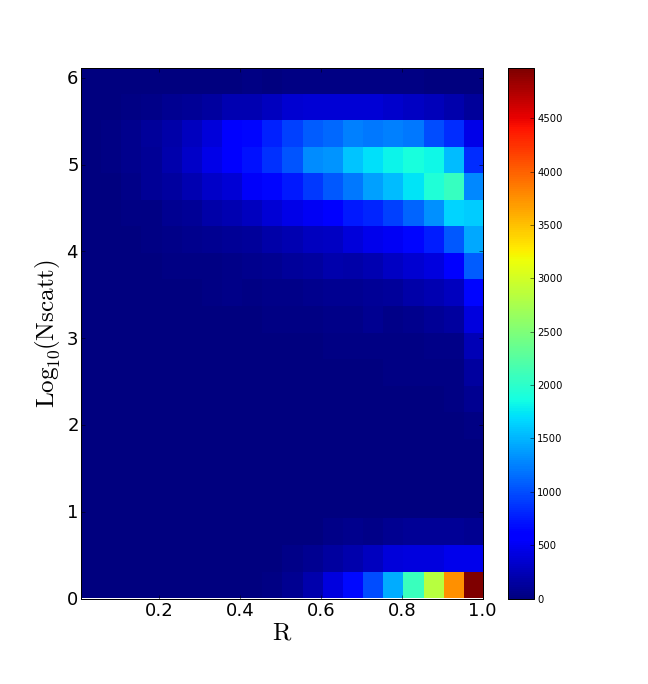
\includegraphics[scale=0.4]{Histogram2dNscattVSRadius.png}
\end{figure}

\end{document}